\documentclass{beamer}

\usetheme{Copenhagen}
\usepackage[utf8]{inputenc}
\usepackage{graphics}

% Slayt basliklarinda kullanilan font boyutu
\setbeamerfont{frametitle}{size=\normalsize}

\title{BM607 DIP2}
\author{Nurettin Şenyer}
\date{2011}
\institute[Ceng]{19/x}

\begin{document}

\frame{\titlepage}

\frame {
	\frametitle{Kavramlar}

	\begin{itemize}
		\item $f(x,y)$, zuaysal koordinat, parlaklık, ayrık değerli - sayısal
		görüntü
		\item piksel: görüntü elemanı; piksel
	\end{itemize}
}

\frame {
	\frametitle{Görüntüleri Neden İşleriz?}
	\begin{itemize}
		\item Resmi elde ederken
			\begin{itemize}
				\item aperturu düzeltmek ve renk dengeleme
				\item yansıtmadan resmi yeniden oluşturma: 3d=>2d, 2d=>3d
			\end{itemize}

		\item Gösterirken veya yazarken
			\begin{itemize}
				\item resim boyutunu ayarlama
				\item binary yazıcılar için halftoning
			\end{itemize}

		\item Saklar ve iletirken
			\begin{itemize}
				\item sayısal kamerada resmi etkin saklama
				\item Mars'dan Dünyaya resim gönderme
			\end{itemize}

		\item Resimleri iyileştirme ve onarma
			\begin{itemize}
				\item eski filimlerden çizikleri giderme
				\item mr'da tümörün görünürlüğünü arttırma
			\end{itemize}

		\item Resimden bilgi çıkartma
			\begin{itemize}
				\item mektuptan posta kodunu okuma
				\item ilaçtan barcodu/qr-kodu okuma
				\item havai resimlerden su kirliliğini ölçme
			\end{itemize}

	\end{itemize}
}
\frame {
	\frametitle{Dalgaboyu}
	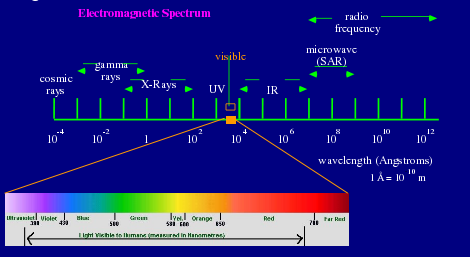
\includegraphics[width=0.9\textwidth]{img/17-wavelength.png}
}
\frame {
	\frametitle{Ölçek: büyük}
	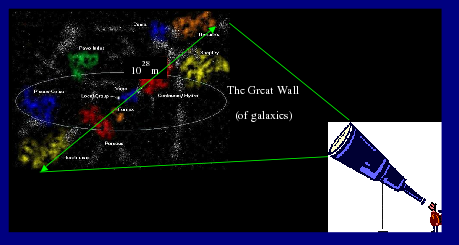
\includegraphics[width=0.9\textwidth]{img/18-olcek-buyuk.png}
}

\frame {
	\frametitle{Ölçek: orta}
	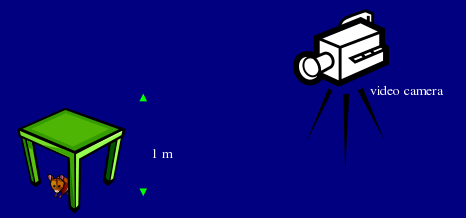
\includegraphics[width=0.9\textwidth]{img/18-olcek-orta.png}
}
\frame {
	\frametitle{Ölçek: küçük}
	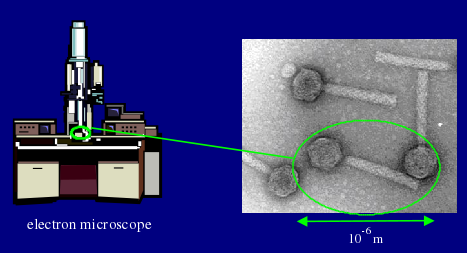
\includegraphics[width=0.9\textwidth]{img/18-olcek-kucuk.png}
}
\frame {
	\frametitle{Resim: biçim}
	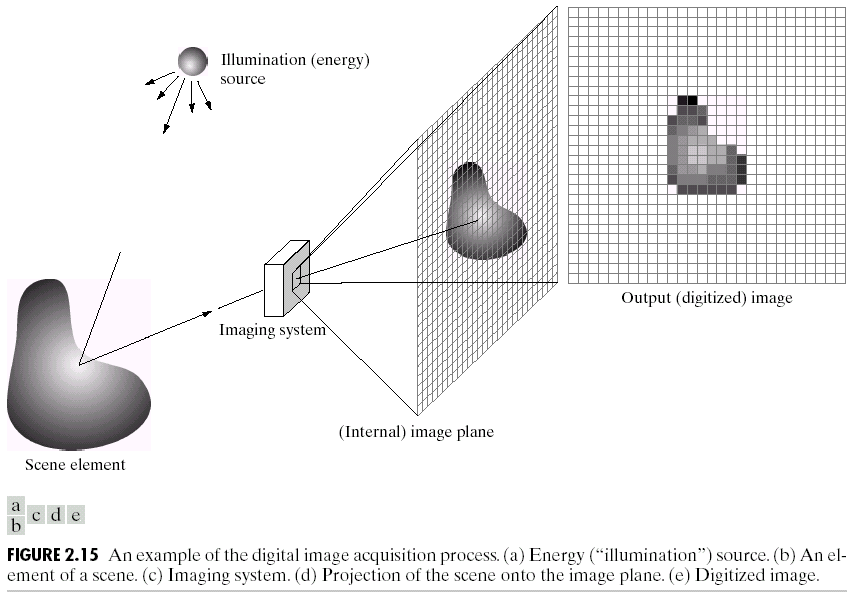
\includegraphics[width=0.9\textwidth]{img/19-image-form.png}
}
\frame {
	\frametitle{Resim: matris}
	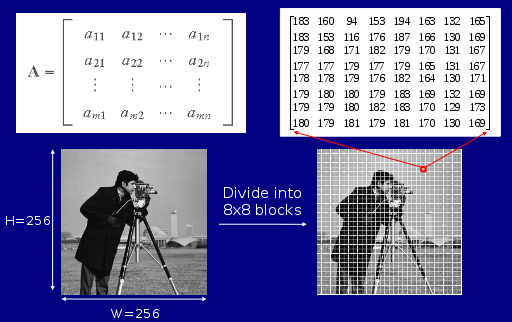
\includegraphics[width=0.9\textwidth]{img/19-matrix-form.png}
}
\frame {
	\frametitle{Çözünürlük}
	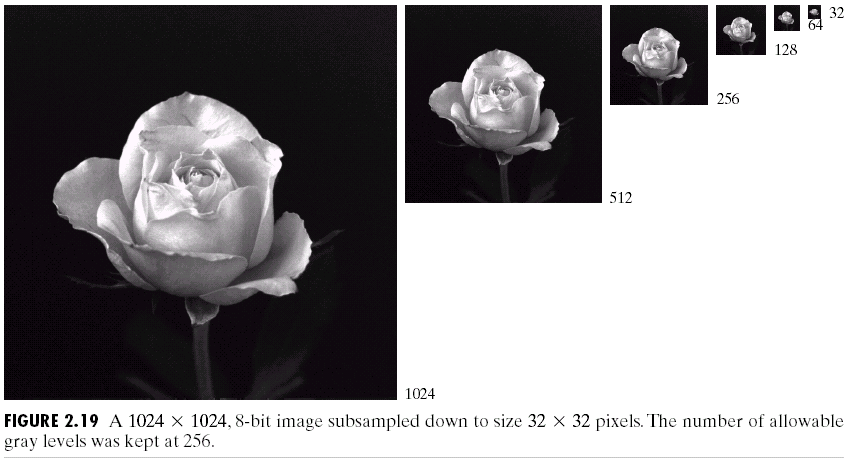
\includegraphics[width=0.9\textwidth]{img/20-resolution.png}
}
\frame {
	\frametitle{Çözünürlük}
	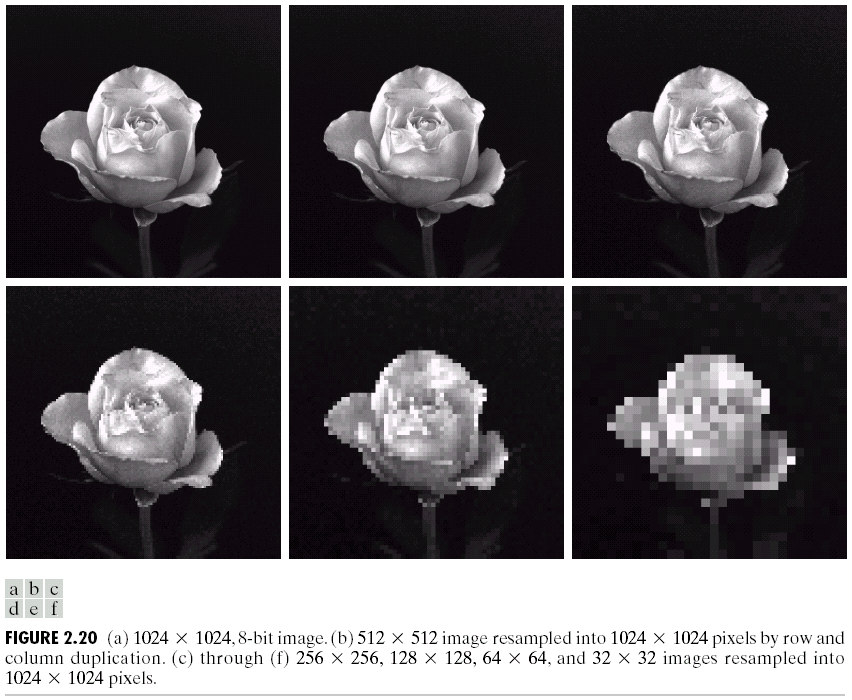
\includegraphics[width=0.9\textwidth]{img/20-resolution2.png}
}
\frame {
	\frametitle{Bitplane}
	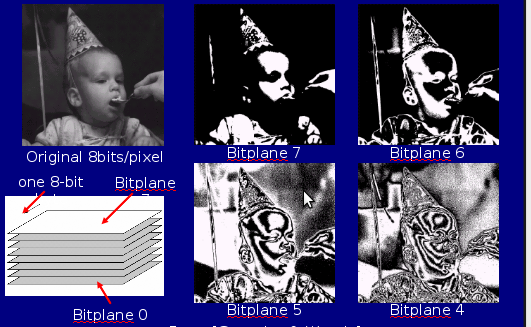
\includegraphics[width=0.9\textwidth]{img/21-bitplane.png}
}
\frame {
	\frametitle{Bitplane}
	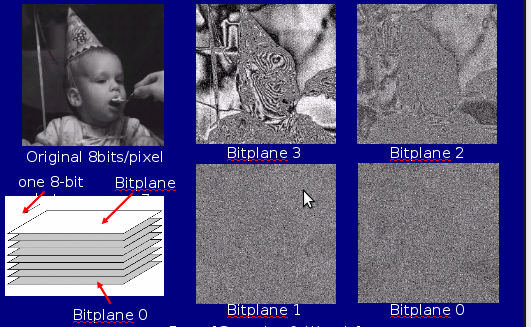
\includegraphics[width=0.9\textwidth]{img/21-bitplane2.png}
}
\frame {
	\frametitle{boyut}
	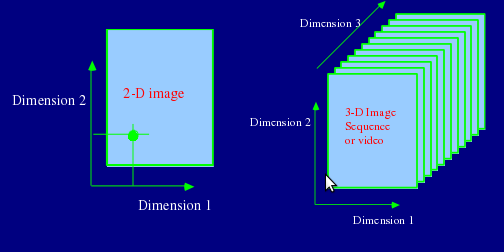
\includegraphics[width=0.9\textwidth]{img/22-dimensionality.png}
}
\frame {
	\frametitle{HVS}
	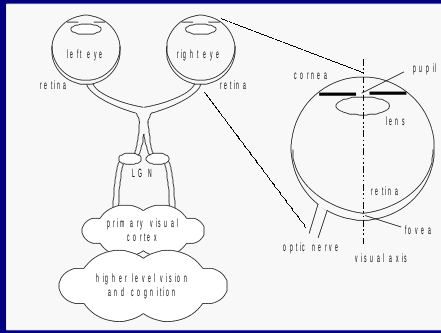
\includegraphics[width=0.9\textwidth]{img/23-hvs.png}
}
\frame {
	\frametitle{renk}
	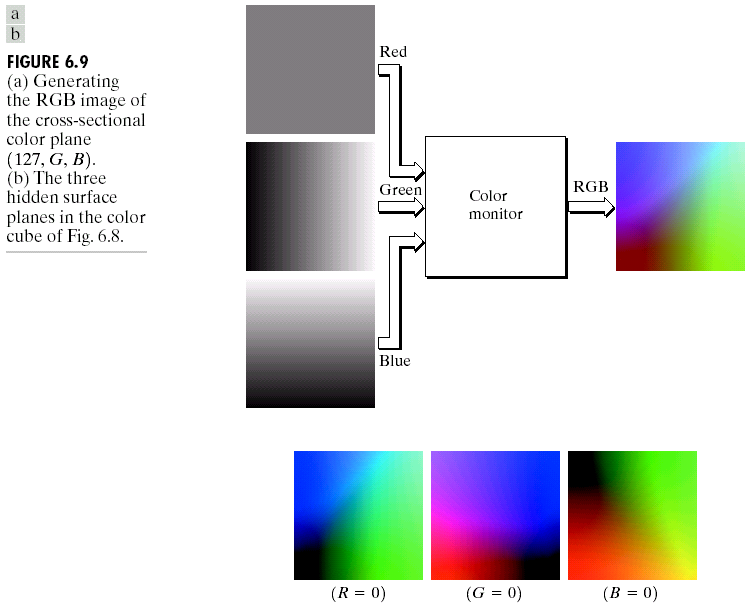
\includegraphics[width=0.9\textwidth]{img/24-renk.png}
}
\frame {
	\frametitle{DIP-1}
	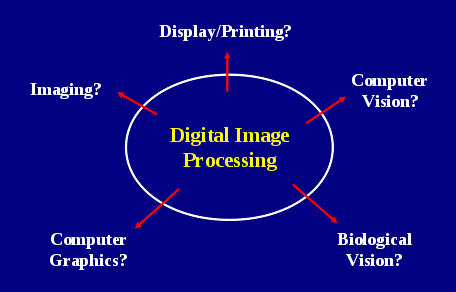
\includegraphics[width=0.9\textwidth]{img/25-dip.png}
}
\frame {
	\frametitle{DIP-2}
	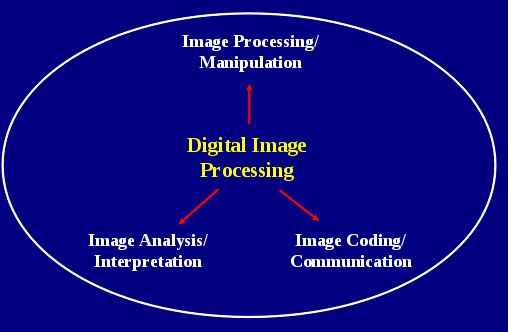
\includegraphics[width=0.9\textwidth]{img/25-dip2.png}
}
\frame {
	\frametitle{DIP-3}
	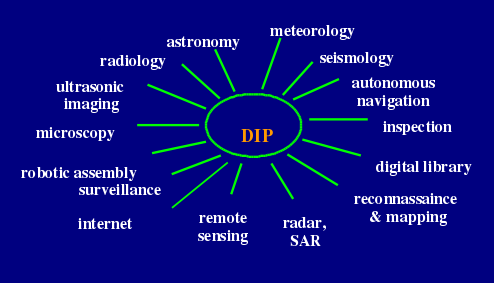
\includegraphics[width=0.9\textwidth]{img/25-dip3.png}
}

\frame {
	\frametitle{Kapsama alanı}

	\begin{itemize}
		\item girişi ve çıkışı resimse - DIP; daraltmaya gerek yok
		\item seviye: görüntü işleme - görüntü analizi - bilgisayarla görü
		\item işleme: gürültü azaltma, zıtlık iyileştirme, netleştirme;
		giriş-çıkışı resim
		\item analiz: bölütleme, dönüşüm, sınıflandırma; giriş-resim,
		çıkış-özellik
		\item görü: nesneleri algılama ve bilişsel işlevler
	\end{itemize}
}

\frame {
	\frametitle{Örnek: OCR}

	\begin{itemize}
		\item metni içeren alanı taramak
		\item önişleme: gürültü giderimi, binarizasyon
		\item bölütleme: karakter çıkarımı
		\item öznitelik çıkarımı
		\item tanıma
	\end{itemize}
}

\frame {
	\frametitle{Görüntüleri Neden İşleriz?}
	\begin{itemize}
		\item Resmi elde ederken
			\begin{itemize}
				\item aperturu düzeltmek ve renk dengeleme
				\item yansıtmadan resmi yeniden oluşturma: 3d=>2d, 2d=>3d
			\end{itemize}

		\item Gösterirken veya yazarken
			\begin{itemize}
				\item resim boyutunu ayarlama
				\item binary yazıcılar için halftoning
			\end{itemize}

		\item Saklar ve iletirken
			\begin{itemize}
				\item sayısal kamerada resmi etkin saklama
				\item Mars'dan Dünyaya resim gönderme
			\end{itemize}

		\item Resimleri iyileştirme ve onarma
			\begin{itemize}
				\item eski filimlerden çizikleri giderme
				\item mr'da tümörün görünürlüğünü arttırma
			\end{itemize}

		\item Resimden bilgi çıkartma
			\begin{itemize}
				\item mektuptan posta kodunu okuma
				\item ilaçtan barcodu/qr-kodu okuma
				\item havai resimlerden su kirliliğini ölçme
			\end{itemize}

	\end{itemize}
}
\frame {
	\frametitle{Onarma}
	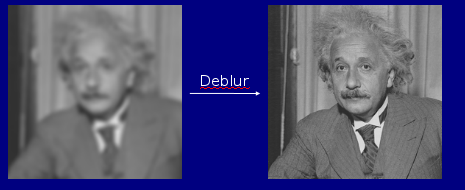
\includegraphics[width=0.9\textwidth]{img/27-onarma.png}
}
\frame {
	\frametitle{Hubble Uzay Teleskobundan alınan resmin onarımı}
	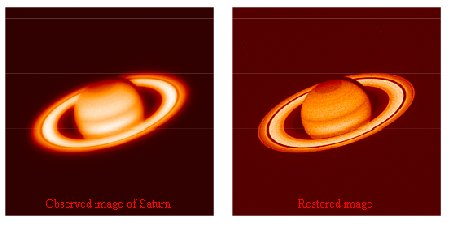
\includegraphics[width=0.9\textwidth]{img/01-onarim.png}
}

\frame {
	\frametitle{İyileştirme}
	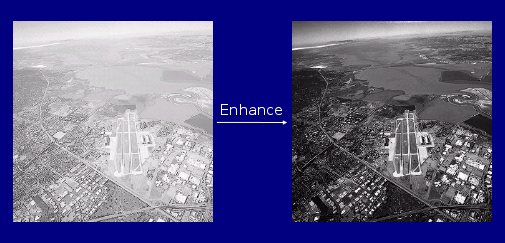
\includegraphics[width=0.9\textwidth]{img/26-iyilestirme.png}
}
\frame{
	\frametitle{Renkli resim iyileştirme}
	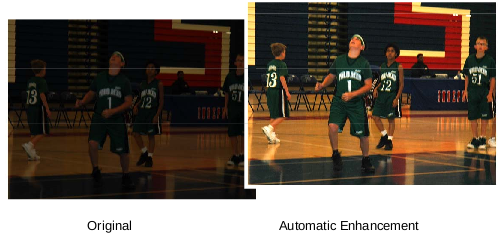
\includegraphics[width=0.9\textwidth]{img/02-renk-iyilestirme.png}
}

\frame{
	\frametitle{Gürültü azaltma}
	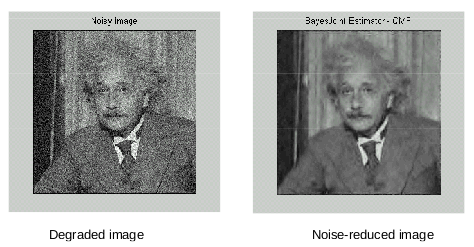
\includegraphics[width=0.9\textwidth]{img/03-gurultu-azaltma.png}
}
\frame{
	\frametitle{Özel efektler}
	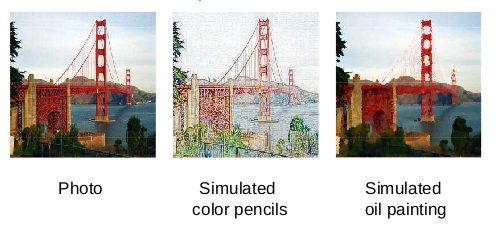
\includegraphics[width=0.9\textwidth]{img/04-ozel-efekt.png}
}
\frame {
	\frametitle{Inpainting}
	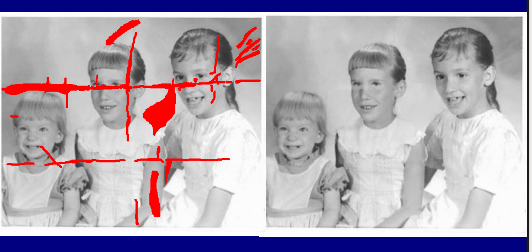
\includegraphics[width=0.9\textwidth]{img/27-inpainting.png}
}
\frame{
	\frametitle{Halftoning}
	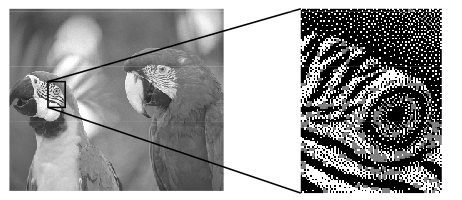
\includegraphics[width=0.9\textwidth]{img/05-halftoning.png}
}
\frame{
	\frametitle{Sözde renkler}
	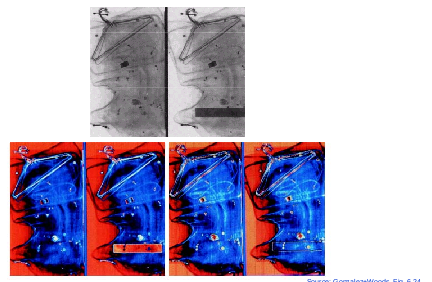
\includegraphics[width=0.9\textwidth]{img/06-pseudo-color.png}
}
\frame{
	\frametitle{Havai resimler}
	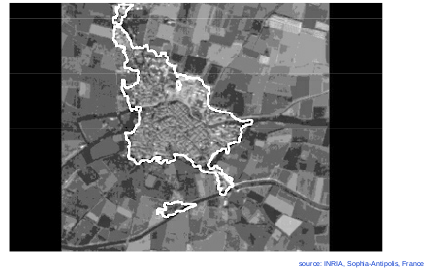
\includegraphics[width=0.9\textwidth]{img/07-aerial-photo.png}
}
\frame{
	\frametitle{Uzaydan deprem araştırması}
	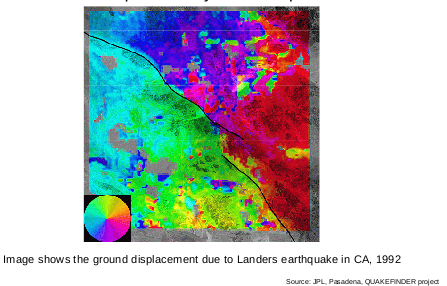
\includegraphics[width=0.9\textwidth]{img/08-earthquake.png}
}
\frame{
	\frametitle{Yüz algılama}
	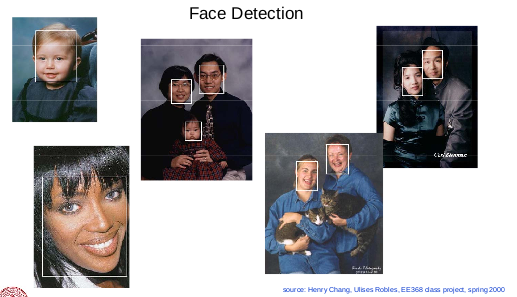
\includegraphics[width=0.9\textwidth]{img/09-face-detection.png}
}
\frame{
	\frametitle{Bölütleme}
	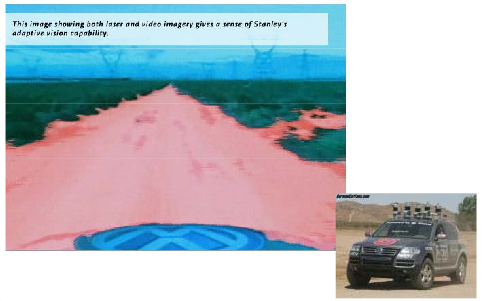
\includegraphics[width=0.9\textwidth]{img/10-segmentation.png}
}
\frame{
	\frametitle{Mozaikler}
	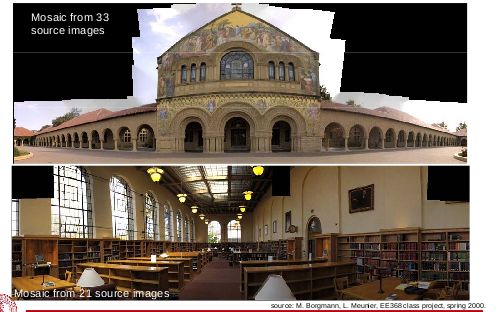
\includegraphics[width=0.9\textwidth]{img/11-mosaic.png}
}
\frame{
	\frametitle{Biçim bozma/dönüştürme}
	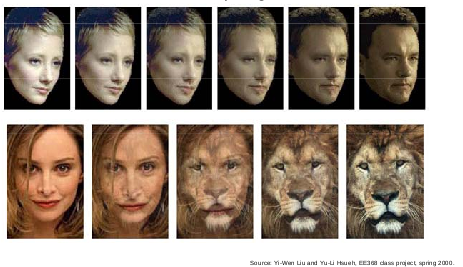
\includegraphics[width=0.9\textwidth]{img/12-morph.png}
}
\frame {
	\frametitle{fextract}
	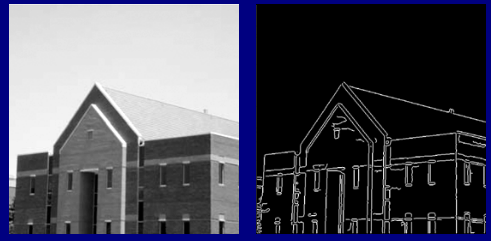
\includegraphics[width=0.9\textwidth]{img/28-edge-detection.png}
}
\frame {
	\frametitle{Bölütleme}
	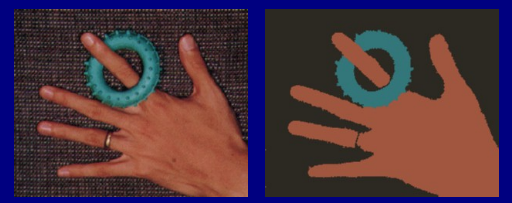
\includegraphics[width=0.9\textwidth]{img/29-bolutleme.png}
}
\frame{
	\frametitle{OCR}
	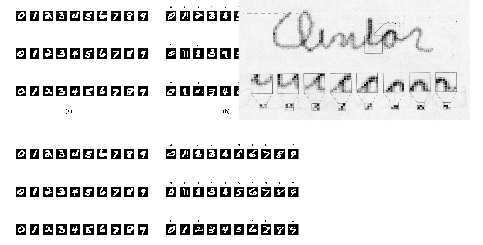
\includegraphics[width=0.9\textwidth]{img/13-ocr.png}
}
\frame{
	\frametitle{Biometrik: parmakizi}
	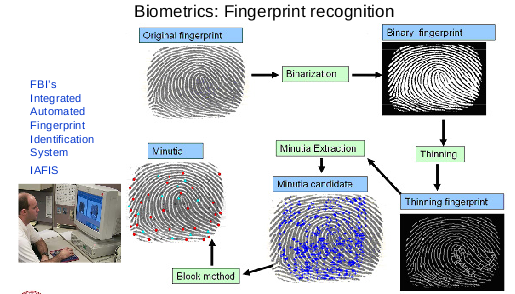
\includegraphics[width=0.9\textwidth]{img/14-fingerprint.png}
}
\frame{
	\frametitle{Biometrik: iris}
	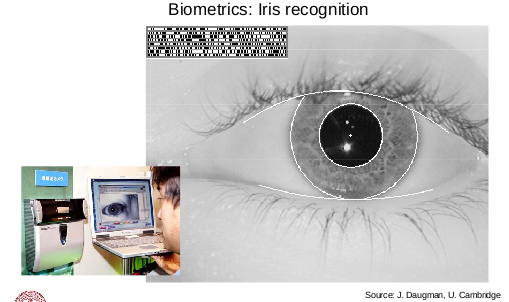
\includegraphics[width=0.9\textwidth]{img/15-iris.png}
}
\frame{
	\frametitle{Qr-kodlar}
	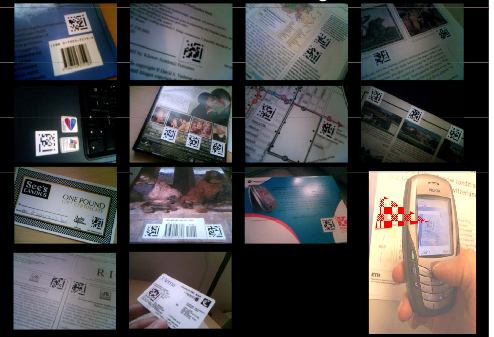
\includegraphics[width=0.9\textwidth]{img/16-qrcode.png}
}
\end{document}
